\documentclass[Main.tex]{subfiles}

\begin{document}
%TODO Voorbeelden geven?
\section{Dataset}

Zoals reeds in de introductie aangehaald is geweest is er op het moment van schrijven geen bestaande dataset die geschikt is voor het onderzochte probleem. Aangezien het noodszakelijk is om te experimenteren op de verschillende aanpakken die hierboven beschreven staan, is er nood aan zelfgegenereerde datasets. Er zijn verschillende manieren om datasets te genereren die ongeveer voldoen aan de vereisten voor het algoritme.
  
\subsection{Verschillende randomgeneratoren}
\subsubsection*{Volledig willekeurig}
Elke waarde die gegenereerd is is een willekeurig getal tussen 0 en 100. Het voordeel aan deze generator is het feit dat er op geen enkele manier een voordeel wordt gegeven aan een bepaald algoritme om deze dataset op te lossen. Nadelig is het feit dat er weinig tot geen structuur zit in een willekeurige reeks van getallen, laat dat net hetgene zijn waar door het algoritme gezocht wordt.

\subsubsection*{Gestructureerd}
De doelwaarde van deze datasets wordt bepaald door een willekeurige vergelijking die bestaat uit de door de gebruiker gegeven operatoren en de waarden die reeds gegenereerd waren op een willekeurige manier. Voordelig hieraan is dat er altijd een oplossing is voor deze datasets, indien alle mogelijkheid van de boom ge\"evalueerd worden. Het feit dat er altijd een oplossing gevonden wordt, toont aan dat er een bepaald voordeel gegeven wordt aan hoe het algoritme momenteel bestaat.

\subsubsection*{Complex gestructureerd}
Hierbij worden de doelwaarden van de willekeurige gegenereerde dataset bepaald door een willekeurige combinatie van willekeurige operaties tussen de reeds willekeurig bepaalde dataset en de constante waarden. Indien de doelwaarde voor deze eerste vergelijking is bepaald, wordt de vergelijking gebruikt om mogelijk meerder voorbeelden van dezelfde vergelijking te bekomen. 

\begin{center}
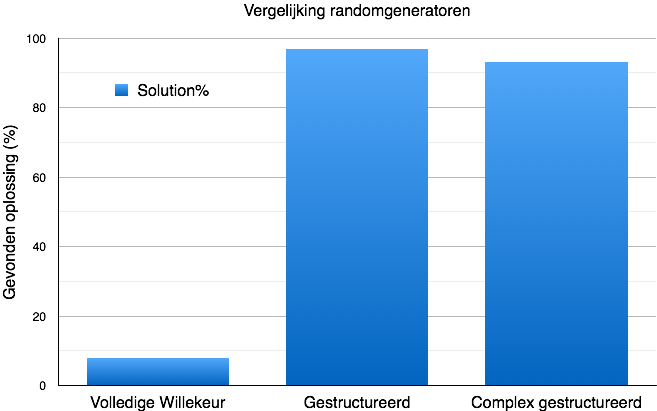
\includegraphics[width=\columnwidth]{compGene.png}
\end{center}

\subsection{Verantwoording keuze}
Om de meeste geschikte datagenerator te bepalen is er een vergelijking nodig tussen de datasets die gecre\"eerd worden door de verschillende generatoren. Het criteria waaraan voldaan moet worden is dat de gegenereerde dataset zo dicht mogelijk bij re\"ele gebruikersdata moet liggen. Er wordt dus vergeleken in hoeveel van de gevallen er op een brute-force manier een oplossing zou gevonden worden in de genereerde dataset. Hierbij bleek dat de \textit{$3^{e}$ datagenerator} de meest geschikte was om gebruikersdata na te bootsen. Alle experimenten die van hieraf aan beschreven staan zijn gebeurd met datasets gegenereerd door deze datagenerator.



\end{document}